\documentclass[10pt]{beamer}
\usetheme{jambro}

\title[]{Mercado de Trabalho}
\author[]{Paulo Victor da Fonseca}
\date{09 de maio de 2023}

\hypersetup{
    colorlinks = true,
    urlcolor = teal,
    linkcolor = teal    
}
\usepackage[portuguese]{babel}
\usepackage{subfig}
\usepackage{emoji}
\usepackage{hyperref}

\begin{document}

\begin{frame}[plain]
    \titlepage{
        \begin{center}
            \begin{minipage}{0.8\textwidth}
                \centering
            \end{minipage}
        \end{center}}
\end{frame}

\begin{frame}{Sumário}
    \tableofcontents
\end{frame}

\section{Introdução}
\begin{frame}
    {Introdução}
    \begin{itemize}
        \item Até agora: preços constantes $\Rightarrow$ firmas capazes e dispostas a ofertar qualquer montante de produto a um dado nível de preços\bigskip
        \item Hipótese aceitável para \textcolor{purple}{curto prazo}\bigskip
        \item \hlight{Médio prazo}: hipótese de $\bar{P}$ deve ser abandonada - explorar ajustes de preços e salários ao longo do tempo e determinar como isso afeta produto agregado\bigskip
        \item Formularemos um modelo para \hlight{mercado de trabalho}, no qual salários são determinados
    \end{itemize}
\end{frame}

\begin{frame}
    {Introdução}
    \begin{figure}
        \centering
        \href{https://www.core-econ.org/the-economy/book/text/09.html}{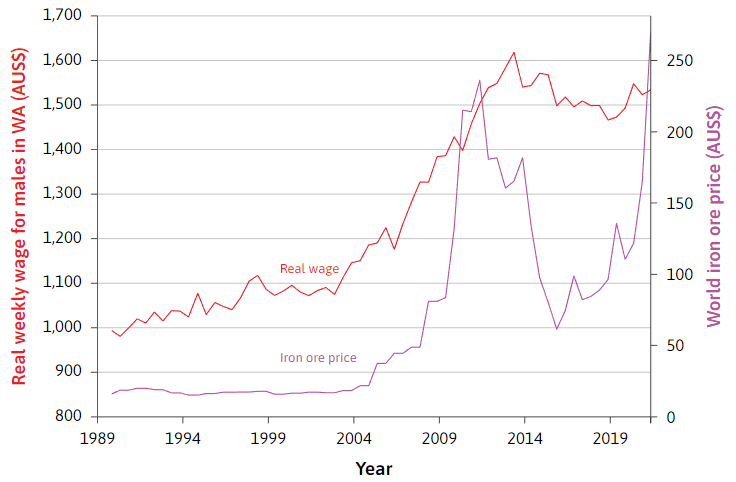
\includegraphics[width=0.65\textwidth]{./figures/aula10_fig1.PNG}}
        \caption{Salário real $\times$ preço do minério de ferro - Western Australia. Fonte: \href{https://www.core-econ.org/the-economy/book/text/09.html}{CORE-Econ}}
    \end{figure}
\end{frame}


\begin{frame}
    {Introdução}
    \begin{figure}
        \centering
        \href{https://www.core-econ.org/the-economy/book/text/09.html}{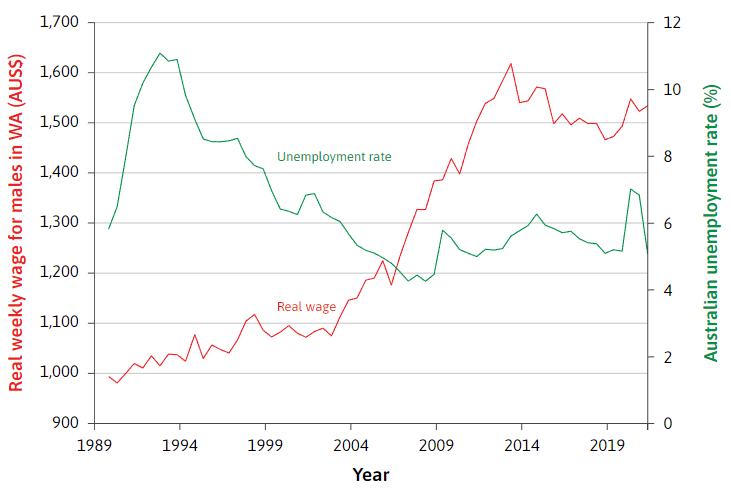
\includegraphics[width=0.6\textwidth]{./figures/aula10_fig2.PNG}}
        \caption{Salário real $\times$ taxa de desemprego - Western Australia. Fonte: \href{https://www.core-econ.org/the-economy/book/text/09.html}{CORE-Econ}}
    \end{figure}
\end{frame}

\section{Mercado de Trabalho}
\begin{frame}{Mercado de Trabalho}
    \begin{itemize}
        \item Começaremos a descrever funcionamento dos mercados de trabalho\bigskip
        \item Por que, mesmo em equilíbrio, a oferta de trabalho excede a demanda por trabalho?\bigskip
        \item Nessas condições: \hlight{desemprego involuntário} ($\times$ desemprego voluntário/friccional)\bigskip
        \item \href{http://www.ilo.org/}{Organização Internacional do Trabalho (OIT)} - definição padronizada de desempregado como pessoas que:\medskip
        \begin{enumerate}
            \item estavam sem trabalho durante um período de referência (usualmente 4 semanas) - não estavam em emprego com carteira assinada ou como autônomo\medskip
            \item estavam disponíveis para trabalhar\medskip
            \item estavam procurando emprego - ativamente tomaram medidas naquele período para encontrar trabalho (carteira assinada ou autônomo)
        \end{enumerate}
    \end{itemize}
\end{frame}

\begin{frame}
    {Mercado de Trabalho}
    \begin{figure}
        \centering
        \href{https://www.core-econ.org/the-economy/book/text/09.html}{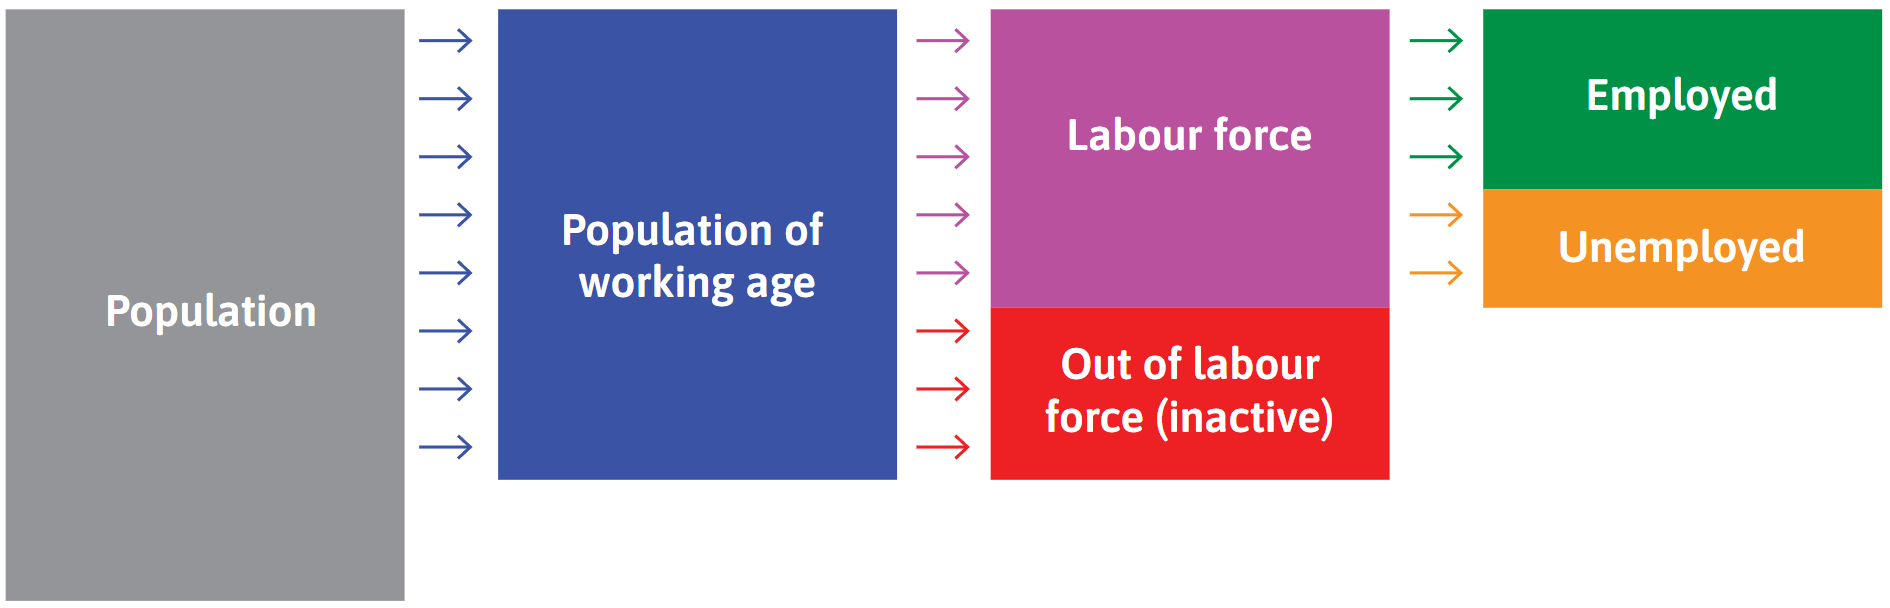
\includegraphics[width=\textwidth]{./figures/aula10_fig3.PNG}}
        \caption{Mercado de Trabalho. Fonte: \href{https://www.core-econ.org/the-economy/book/text/09.html}{CORE-Econ}}
    \end{figure}
\end{frame}

\begin{frame}{Mercado de Trabalho}
    \begin{center}
		\begin{minipage}[b]{.55\textwidth}
			\begin{tikzpicture}
				\node[inner sep=0, align=left] (image) at (0,0) {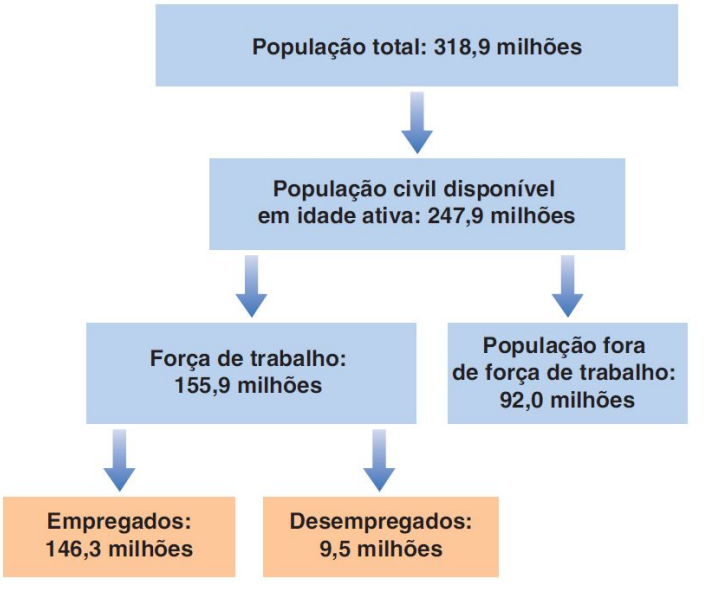
\includegraphics[width=\textwidth]{./figures/aula10_fig4.PNG}};					
			\end{tikzpicture}
			\tiny{{\scshape FIGURA}. \ Mercado de Trabalho - EUA 2014 (em milhões). Fonte: Blanchard (2017)} 
		\end{minipage}
	\end{center}
\end{frame}

\begin{frame}{Mercado de Trabalho}
    \begin{center}
		\begin{minipage}[b]{.55\textwidth}
			\begin{tikzpicture}
				\node[inner sep=0, align=left] (image) at (0,0) {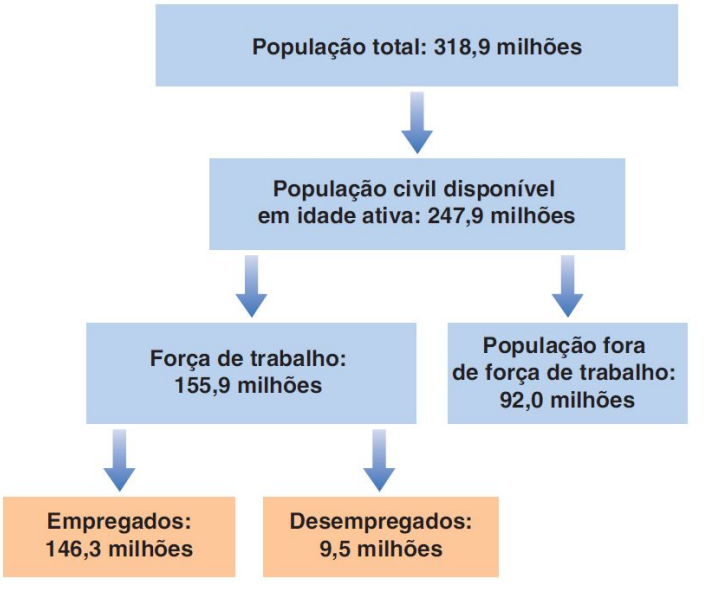
\includegraphics[width=\textwidth]{./figures/aula10_fig4.PNG}};
				\draw[arrow,->,opacity=1] (2.5,1.3) to[bend left] +(+1,+0) node[anchor=west,opacity=1] {\normalsize{\hand \begin{tabular}{l}
    Exclui: \\
    - < 16 anos \\
    - alistamentos F.A. \\ 
    - população encarcerada
\end{tabular}}};				
			\end{tikzpicture}
			\tiny{{\scshape FIGURA}. \ Mercado de Trabalho - EUA 2014 (em milhões). Fonte: Blanchard (2017)} 
		\end{minipage}
	\end{center}
\end{frame}

\begin{frame}{Mercado de Trabalho}
    \begin{center}
		\begin{minipage}[b]{.55\textwidth}
			\begin{tikzpicture}
				\node[inner sep=0, align=right] (image) at (0,0) {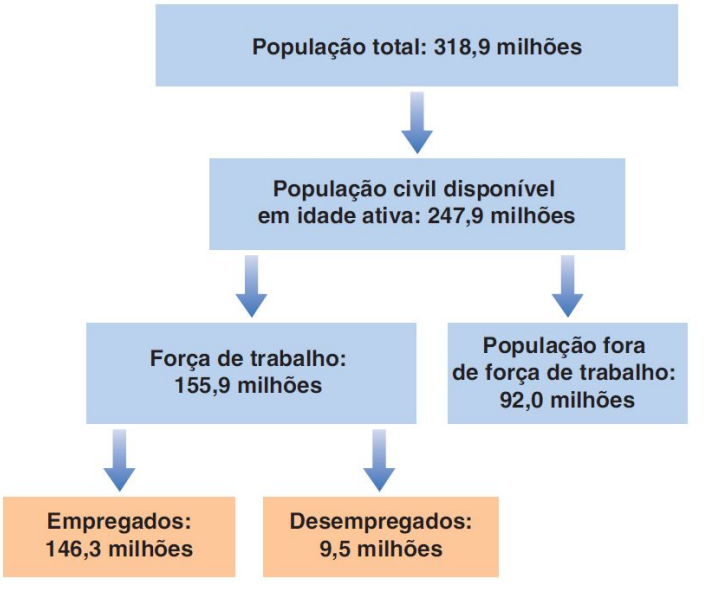
\includegraphics[width=\textwidth]{./figures/aula10_fig4.PNG}};
				\draw[arrow,->,opacity=1] (-1.5,0.3) to[bend right] +(-1,+0) node[anchor=east,opacity=1] {\normalsize{\hand \begin{tabular}{l}
    Taxa de participação: \\
    - F.T./P.I.A. \\
    - 63\%
\end{tabular}}};				
			\end{tikzpicture}
			\tiny{{\scshape FIGURA}. \ Mercado de Trabalho - EUA 2014 (em milhões). Fonte: Blanchard (2017)} 
		\end{minipage}
	\end{center}
\end{frame}

\begin{frame}{Mercado de Trabalho}
    \begin{center}
		\begin{minipage}[b]{.55\textwidth}
			\begin{tikzpicture}
				\node[inner sep=0, align=left] (image) at (0,0) {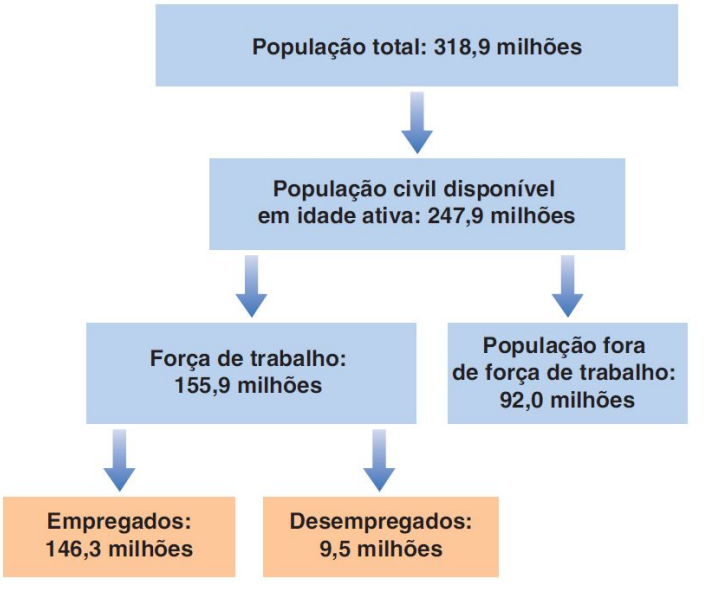
\includegraphics[width=\textwidth]{./figures/aula10_fig4.PNG}};
				\draw[arrow,->,opacity=1] (0.7,-2) to[bend left] +(+1.2,-0.5) node[anchor=west,opacity=1] {\normalsize{\hand \begin{tabular}{l}
    Taxa de desemprego: \\
    - desempregados/F.T. \\
    - 6,1\%
\end{tabular}}};				
			\end{tikzpicture}
			\tiny{{\scshape FIGURA}. \ Mercado de Trabalho - EUA 2014 (em milhões). Fonte: Blanchard (2017)} 
		\end{minipage}
	\end{center}
\end{frame}

\begin{frame}{Mercado de Trabalho}
    \begin{center}
		\begin{minipage}[b]{.55\textwidth}
			\begin{tikzpicture}
				\node[inner sep=0, align=right] (image) at (0,0) {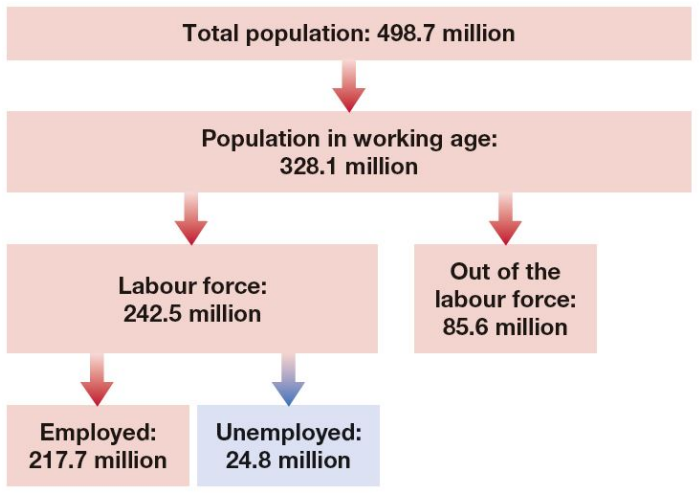
\includegraphics[width=\textwidth]{./figures/aula10_fig5.PNG}};
				\draw[arrow,->,opacity=1,blue] (-2.1,0.4) to[bend right] +(-1,-0.2) node[anchor=east,opacity=1] {\normalsize{\hand \begin{tabular}{l}
    Taxa de participação: \\    
    - 73,9\%
\end{tabular}}};				
			\end{tikzpicture}
			\tiny{{\scshape FIGURA}. \ Mercado de Trabalho - União Europeia 2014 (em milhões). Fonte: Blanchard, Amighini, Giavazzi (2017)} 
		\end{minipage}
	\end{center}
\end{frame}

\begin{frame}{Mercado de Trabalho}
    \begin{center}
		\begin{minipage}[b]{.55\textwidth}
			\begin{tikzpicture}
				\node[inner sep=0, align=left] (image) at (0,0) {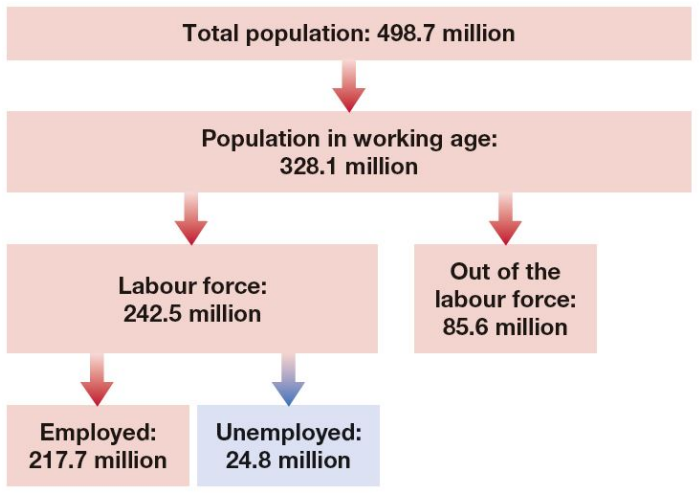
\includegraphics[width=\textwidth]{./figures/aula10_fig5.PNG}};
				\draw[arrow,->,opacity=1,blue] (-0.2,-1.5) to[bend left] +(+1,-0.5) node[anchor=west,opacity=1] {\normalsize{\hand \begin{tabular}{l}
    Taxa de desemprego: \\    
    - 73,9\%
\end{tabular}}};				
			\end{tikzpicture}
			\tiny{{\scshape FIGURA}. \ Mercado de Trabalho - União Europeia 2014 (em milhões). Fonte: Blanchard, Amighini, Giavazzi (2017)} 
		\end{minipage}
	\end{center}
\end{frame}

\begin{frame}{Mercado de Trabalho}
    \begin{center}
		\begin{minipage}[b]{.55\textwidth}
			\begin{tikzpicture}
				\node[inner sep=0, align=left] (image) at (0,0) {\href{https://www.ibge.gov.br/explica/desemprego.php}{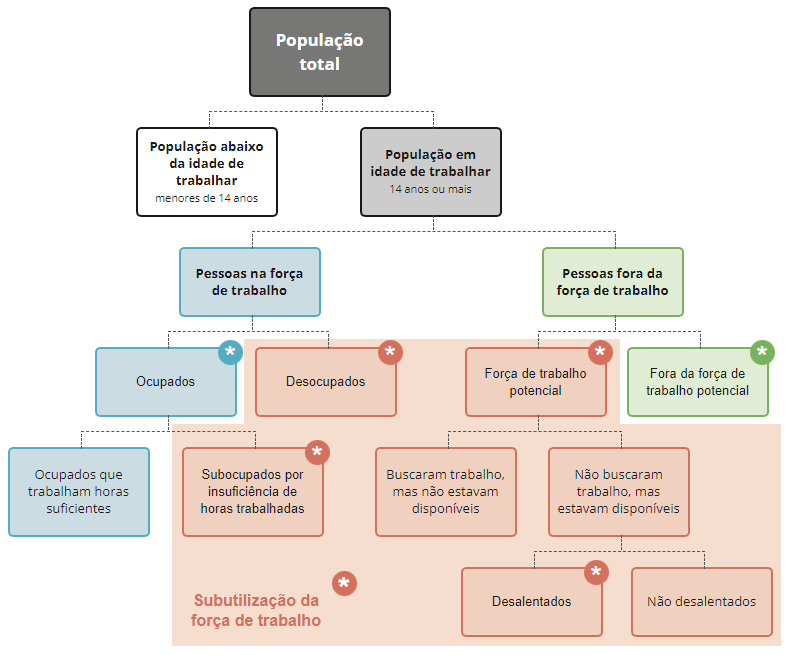
\includegraphics[width=\textwidth]{./figures/aula10_fig6.PNG}}};								
			\end{tikzpicture}
			\tiny{{\scshape FIGURA}. \ Mercado de Trabalho - Classificação IBGE. Fonte: \href{https://www.ibge.gov.br/explica/desemprego.php}{IBGE}} 
		\end{minipage}
	\end{center}
\end{frame}

\begin{frame}{Mercado de Trabalho}
    \begin{center}
		\begin{minipage}[b]{.9\textwidth}
			\begin{tikzpicture}
				\node[inner sep=0, align=left] (image) at (0,0) {\href{https://www.ibge.gov.br/explica/desemprego.php}{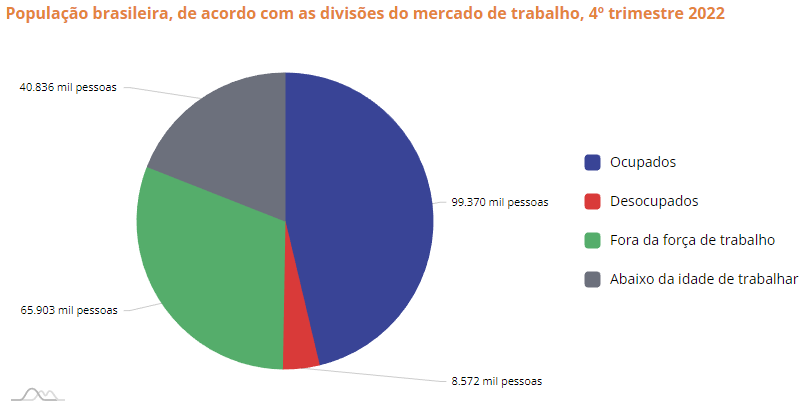
\includegraphics[width=\textwidth]{./figures/aula10_fig7.PNG}}};								
			\end{tikzpicture}
			\tiny{{\scshape FIGURA}. \ Mercado de Trabalho - Brasil (2022.4). Fonte: \href{https://www.ibge.gov.br/explica/desemprego.php}{IBGE}} 
		\end{minipage}
	\end{center}
\end{frame}

\begin{frame}{Mercado de Trabalho}
    \begin{itemize}
        \item Uma dada taxa de desemprego pode refletir realidades bem diversas:\bigskip
        \begin{enumerate}
            \item Mercado de trabalho ativo: muitos \textcolor{purple}{desligamentos} e muitas \textcolor{blue}{admissões}\medskip
            \item Mercado de trabalho \hlight{esclerosado}: poucos desligamentos, poucas admissões e contingente estagnado de desempregados
        \end{enumerate}
    \end{itemize}
\end{frame}

\begin{frame}{Mercado de Trabalho}
\begin{itemize}
		\item \href{https://www.census.gov/programs-surveys/cps.html}{Current Population Survey (CPS) - US Census Bureau}
	\end{itemize}
    \begin{center}
		\begin{minipage}[b]{.45\textwidth}
			\begin{tikzpicture}
				\node[inner sep=0, align=left] (image) at (0,0) {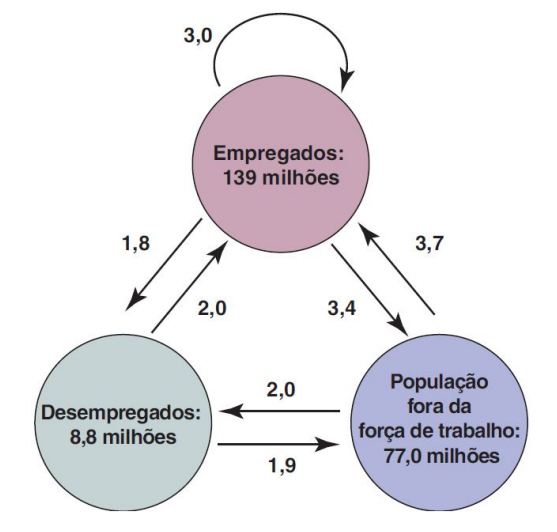
\includegraphics[width=\textwidth]{./figures/aula10_fig8.PNG}};
				\draw[arrow,->,opacity=1] (1.3,1.3) to[bend left] +(+1,+0) node[anchor=west,opacity=1] {\normalsize{\hand \begin{tabular}{l}
    Grandes fluxos: \\
    - 8,2 milhões desligamentos/mês \\
    - 75\% demissões voluntárias \\ 
    - 25\% demissões involuntárias
\end{tabular}}};				
			\end{tikzpicture}
			\tiny{{\scshape FIGURA}. \ Fluxos médios mensais - EUA 1996-2014 (em milhões). Fonte: Blanchard (2017)} 
		\end{minipage}
	\end{center}
\end{frame}

\begin{frame}{Mercado de Trabalho}
\begin{itemize}
		\item \href{https://www.census.gov/programs-surveys/cps.html}{Current Population Survey (CPS) - US Census Bureau}
	\end{itemize}
    \begin{center}
		\begin{minipage}[b]{.45\textwidth}
			\begin{tikzpicture}
				\node[inner sep=0, align=left] (image) at (0,0) {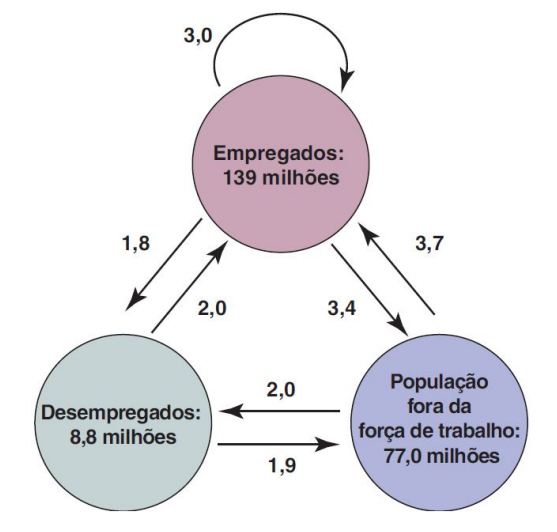
\includegraphics[width=\textwidth]{./figures/aula10_fig8.PNG}};
				\draw[arrow,->,opacity=1, brick] (1.3,1.3) to[bend left] +(+1,+0) node[anchor=west,opacity=1] {\normalsize{\hand \begin{tabular}{l}
    Relação ao \# de desempregados: \\
    - 44\% dos desempregados deixam \\
    essa condição a cada mês \\
    - Duração média desemprego: \\
    2-3 meses
\end{tabular}}};				
			\end{tikzpicture}
			\tiny{{\scshape FIGURA}. \ Fluxos médios mensais - EUA 1996-2014 (em milhões). Fonte: Blanchard (2017)} 
		\end{minipage}
	\end{center}
\end{frame}

\begin{frame}{Mercado de Trabalho}
\begin{itemize}
		\item \href{https://www.census.gov/programs-surveys/cps.html}{Current Population Survey (CPS) - US Census Bureau}
	\end{itemize}
    \begin{center}
		\begin{minipage}[b]{.45\textwidth}
			\begin{tikzpicture}
				\node[inner sep=0, align=left] (image) at (0,0) {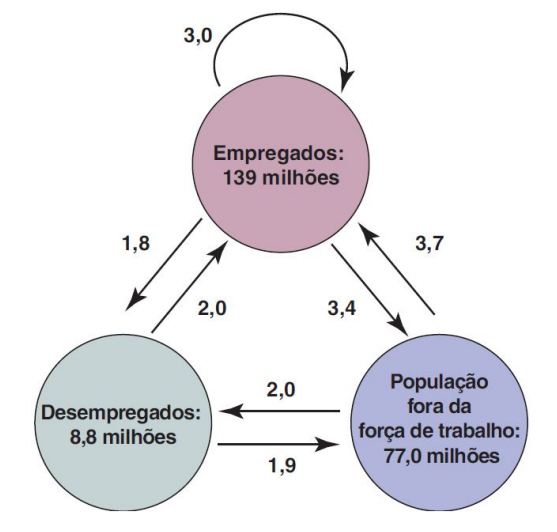
\includegraphics[width=\textwidth]{./figures/aula10_fig8.PNG}};
				\draw[arrow,->,opacity=1, blue] (1.3,1.3) to[bend left] +(+1,+0) node[anchor=west,opacity=1] {\normalsize{\hand \begin{tabular}{l}
    Fluxos elevados in-out F.T.: \\
    \emoji{warning} Trabalhadores desalentados \\    
    - Foco na taxa de emprego
\end{tabular}}};				
			\end{tikzpicture}
			\tiny{{\scshape FIGURA}. \ Fluxos médios mensais - EUA 1996-2014 (em milhões). Fonte: Blanchard (2017)} 
		\end{minipage}
	\end{center}
\end{frame}

\begin{frame}{Mercado de Trabalho}
    \begin{footnotesize}
        \begin{table}[h!]
            \centering
            \begin{tabular}{ |l||c|c|c|c|c|c|c|c|  }
                \hline
                \multicolumn{9}{|c|}{Duração média do desemprego (meses)}                \\
                \hline
                \hline
                País             & 2014 & 2015 & 2016 & 2017 & 2018 & 2019 & 2020 & 2021 \\
                \hline
                \rowcolor{gray!10} Canadá           & 4,3  & 4,1  & 4,1  & 4,1  & 3,8  & 3,5  & 3,3  & 4,9  \\
                Colômbia         & 4,3  & 4,0  & 4,1  & 4,3  & 4,7  & 5,0  & 4,7  & 6,5  \\
                \rowcolor{gray!10} Eslováquia       & 29,6 & 31,5 & 29,1 & 30,2 & 29,8 & 28,5 & 23,8 & 20,6 \\
                Estados Unidos   & 7,8  & 6,7  & 6,3  & 5,8  & 5,2  & 5,0  & 3,8  & 6,6  \\
                \rowcolor{gray!10} Finlândia        & 10,7 & 10,5 & 10,4 & 10,7 & 10,2 & 9,7  & 8,2  & 11,3 \\
                França           & 14,2 & 14,6 & 15,6 & 15,5 & 14,5 & 13,9 & 13,4 & -    \\
                \rowcolor{gray!10} Hungria          & 18,2 & 18,1 & 18,1 & 16,0 & 15,2 & 12,4 & 9,9  & 8,4  \\
                República Tcheca & 17,6 & 19,4 & 18,3 & 15,6 & 14,0 & 13,8 & 10,4 & 11,8 \\
                \rowcolor{gray!10} Suíça            & 16,9 & 17,2 & 17,3 & 17,0 & 18,0 & 17,6 & 16,0 & 17,8 \\
                \hline
            \end{tabular}\vspace{.2cm}\newline
			\tiny{{\scshape TABELA.} Duração média do desemprego em meses. Fonte: \href{https://stats.oecd.org/index.aspx?DataSetCode=AVD_DUR}{OECD.stats}\newline}%
        \end{table}
    \end{footnotesize}
\end{frame}

\begin{frame}{Mercado de Trabalho}
    \begin{center}
		\begin{minipage}[b]{.9\textwidth}
			\begin{tikzpicture}
				\node[inner sep=0, align=left] (image) at (0,0) {\href{https://data.oecd.org/chart/6Rq2}{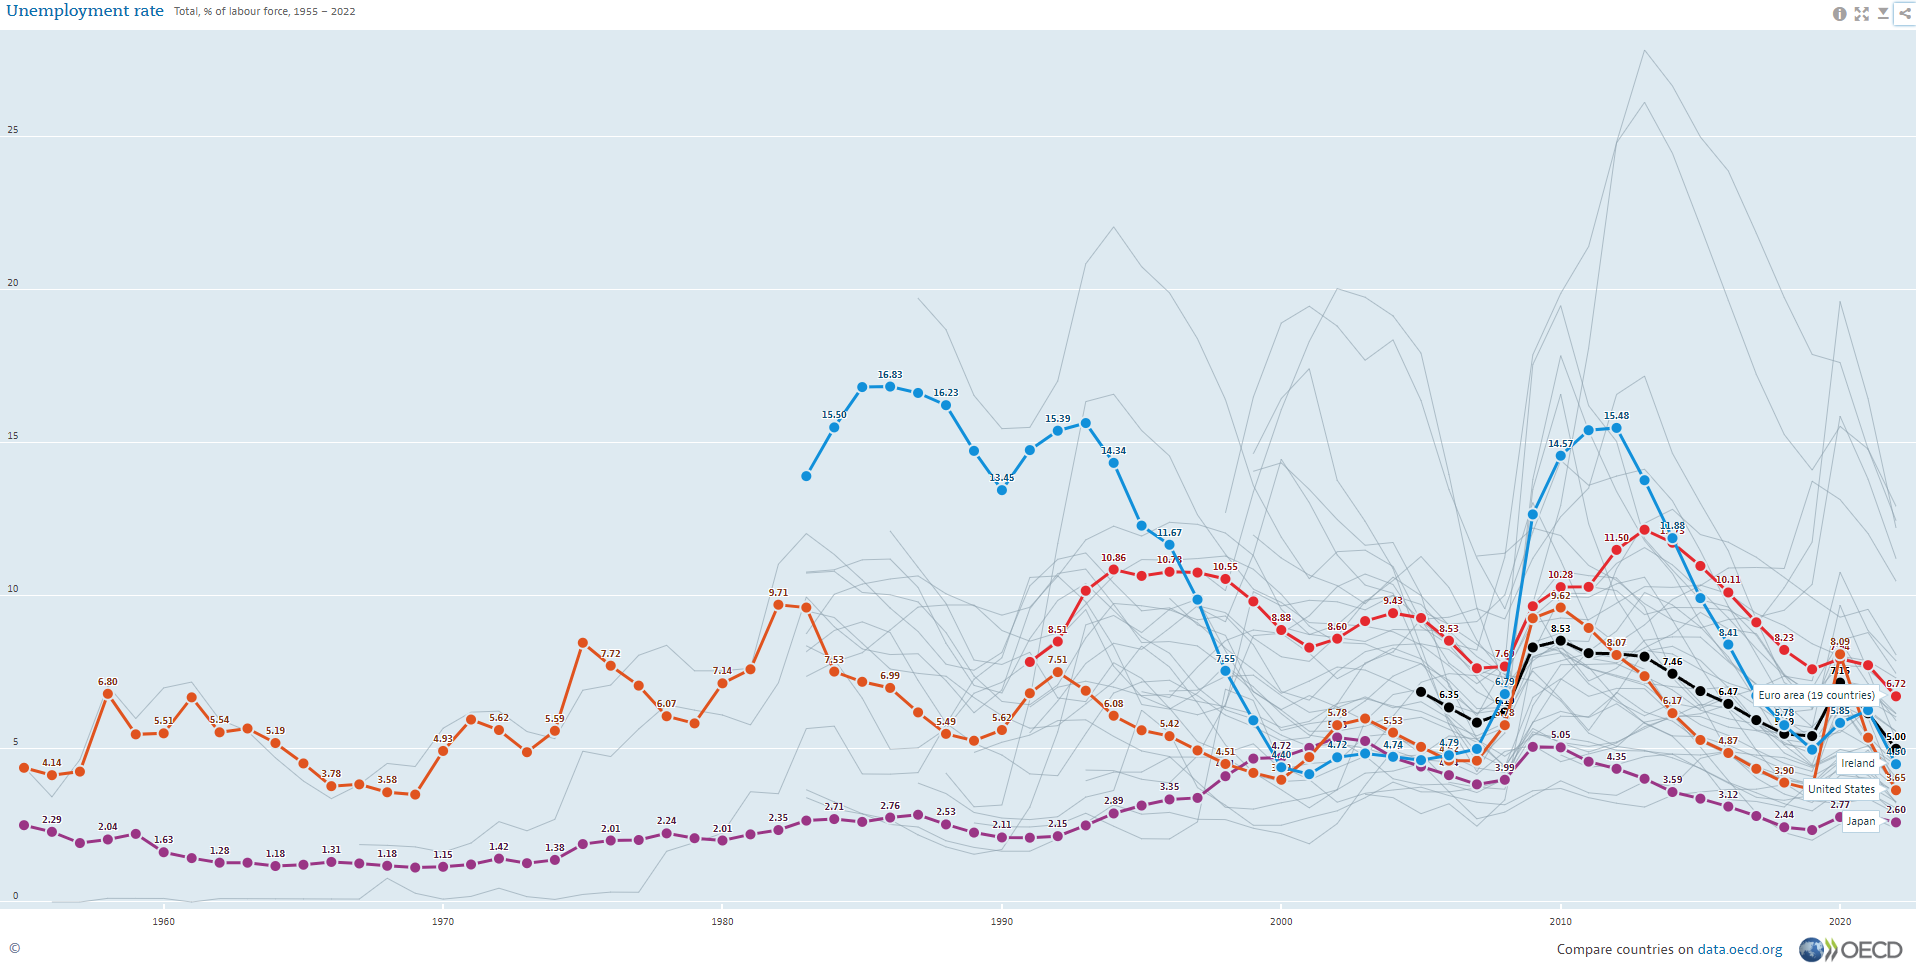
\includegraphics[width=\textwidth]{./figures/aula10_fig9.PNG}}};
			\end{tikzpicture}
			\tiny{{\scshape FIGURA}. \ Tendência e heterogeneidade no desemprego (seleção OCDE): 1955-2022. Fonte: \href{https://data.oecd.org/chart/6Rq2}{OCDE}} 
		\end{minipage}
	\end{center}
\end{frame}

\begin{frame}{Mercado de Trabalho}
    \begin{itemize}
        \item Taxa de desemprego varia ao longo do tempo e entre países\bigskip
        \item Elevado grau de heterogeneidade\bigskip
        \item Pós CFG2008 (entre 2009 e 2012):\medskip
            \begin{itemize}
                \item Holanda: desemprego médio de 4,5\%\medskip
                \item Espanha: desemprego médio de 21,2\%\bigskip
            \end{itemize}
        \item Mesmo país pode apresentar grandes variações ao longo do tempo\bigskip
        \item Irlanda:\medskip
        \begin{itemize}
            \item Desemprego $\approx$ 16\% final dos anos 1980s\medskip
            \item Começo dos anos 2000s, desemprego de $\approx$ 4\%\medskip
            \item Início da crise, aumentando novamente para 14\%
        \end{itemize}
    \end{itemize}
\end{frame}

\section{Dinâmica do Desemprego}
\begin{frame}{Dinâmica do Desemprego}
    \begin{center}
		\begin{minipage}[b]{\textwidth}
			\begin{tikzpicture}
				\node[inner sep=0, align=left] (image) at (0,0) {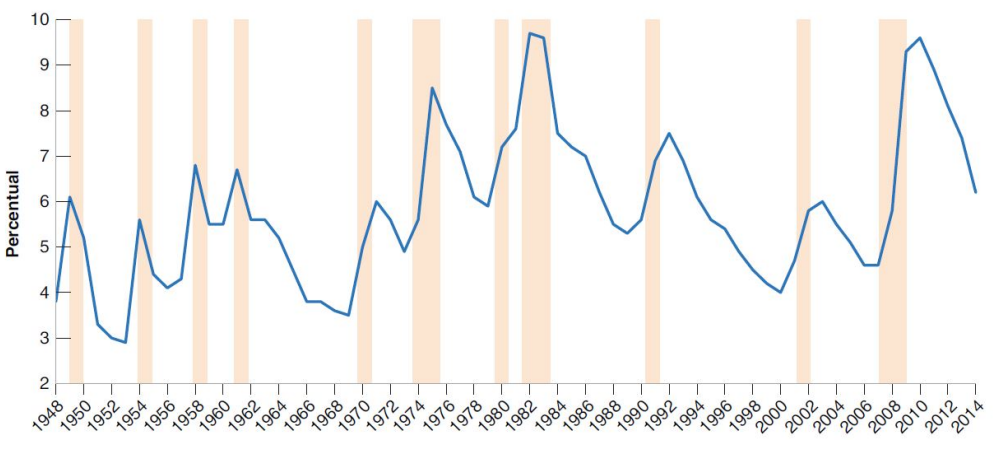
\includegraphics[width=\textwidth]{./figures/aula10_fig10.PNG}};
			\end{tikzpicture}
			\tiny{{\scshape FIGURA}. \ Dinâmica da taxa de desemprego, EUA (1948-2014). Fonte: Blanchard (2017)} 
		\end{minipage}
	\end{center}
\end{frame}

\begin{frame}{Dinâmica do Desemprego}
    \begin{itemize}
        \item Até meados dos 1980s: tendência de alta da taxa de desemprego\medskip
        \begin{itemize}
            \item Década de 1950: média de 4,5\%\medskip
            \item Década de 1960: média de 4,7\%\medskip
            \item Década de 1970: média de 6,2\%\medskip
            \item Década de 1980: média de 7,3\%\medskip
        \end{itemize}
        \item Desde então, taxa de desemprego declinou continuamente por mais de 2 décadas\bigskip
        \item CFG2008: taxa aumentou acentuadamente, mas tornou a baixar de novo
    \end{itemize}
\end{frame}

\begin{frame}{Dinâmica do Desemprego}
    \begin{itemize}
        \item Deixando de lado oscilações de tendência, \hlight{os movimentos anuais da taxa de desemprego estão fortemente associados a recessões e expansões}\bigskip
        \item Desemprego é custoso pois representa subutilização de recursos e, além disso, está associado a infelicidade e estresse psicológico\bigskip
        \item Como flutuações da taxa de desemprego afetam trabalhadores individualmente?\medskip
        \begin{enumerate}
            \item Efeito dos movimentos da taxa de desemprego agregado sobre bem-estar individual dos trabalhadores\medskip
            \item Efeito da taxa de desemprego agregado sobre salários
        \end{enumerate}
    \end{itemize}
\end{frame}

\begin{frame}{Dinâmica do Desemprego}
    \begin{itemize}
        \item Como empresas podem reduzir emprego frente a redução de demanda?\bigskip
        \item Podem frear admissão de novos funcionários ou demitir empregados\bigskip
        \item Normalmente, a primeira opção é preferível (contando com demissões voluntárias ou aposentadorias)\bigskip
        \item Mas pode não ser suficiente se a redução na demanda for grande e, então, empresas podem ter de demitir funcionários
    \end{itemize}
\end{frame}

\begin{frame}{Dinâmica do Desemprego}
    \begin{itemize}
        \item Implicações para empregados e desempregados:\medskip
        \begin{enumerate}
            \item Ajuste via número menor de admissões: probabilidade de desempregado encontrar emprego diminuirá - menos admissões $\Rightarrow$ menor abertura de postos de trabalho e maior desemprego $\Rightarrow$ mais candidatos para postos de trabalho\medskip
            \item Ajuste via demissões involuntárias: empregados terão risco maior de perder seus empregos\bigskip
        \end{enumerate}
        \item De modo geral, empresas recorrem às duas formas de ajuste - desemprego maior relacionado tanto com probabilidade menor de desempregados encontrarem emprego quanto probabilidade maior de empregados perderem o emprego
    \end{itemize}
\end{frame}

\begin{frame}{Dinâmica do Desemprego}
    \begin{center}
		\begin{minipage}[b]{.9\textwidth}
			\begin{tikzpicture}
				\node[inner sep=0] (image) at (0,0) {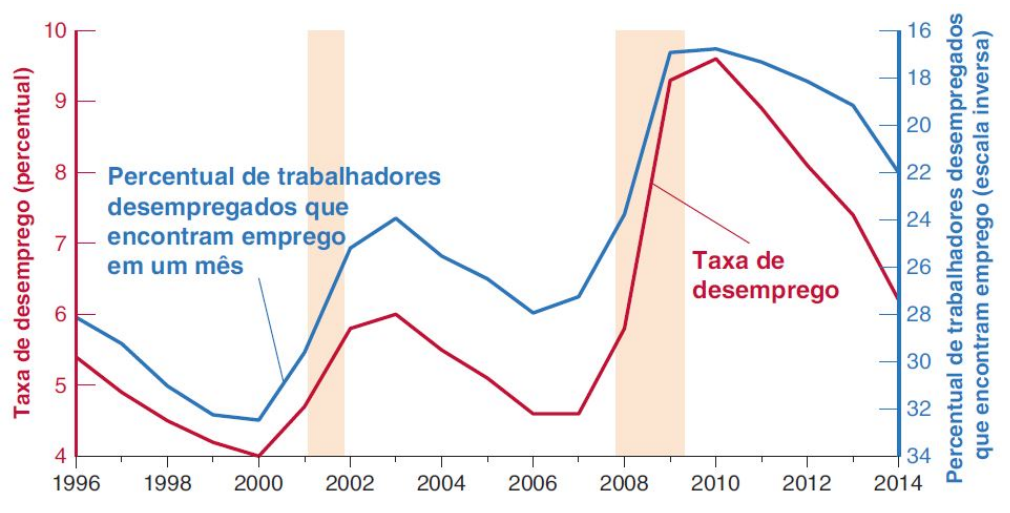
\includegraphics[width=\textwidth]{./figures/aula10_fig11.PNG}};
			\end{tikzpicture}
			\tiny{{\scshape FIGURA}. \ Taxa de desemprego e proporção de desempregados que encontram emprego, EUA (1996-2014). Fonte: Blanchard (2017)} 
		\end{minipage}
	\end{center}
\end{frame}

\begin{frame}{Dinâmica do Desemprego}
    \begin{center}
		\begin{minipage}[b]{.9\textwidth}
			\begin{tikzpicture}
				\node[inner sep=0] (image) at (0,0) {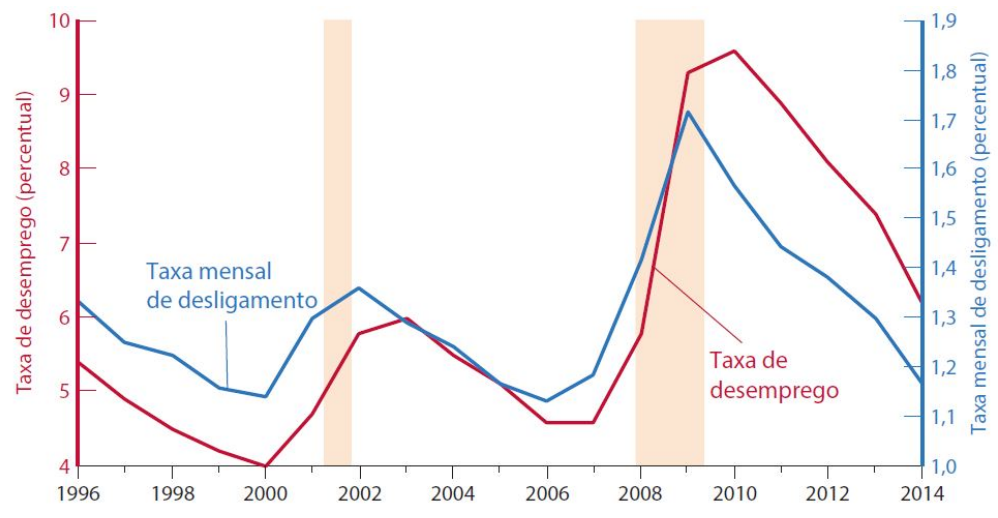
\includegraphics[width=\textwidth]{./figures/aula10_fig12.PNG}};
			\end{tikzpicture}
			\tiny{{\scshape FIGURA}. \ Taxa de desemprego e taxa mensal de desligamento, EUA (1996-2014). Fonte: Blanchard (2017)} 
		\end{minipage}
	\end{center}
\end{frame}

\begin{frame}{Dinâmica do Desemprego}
    \begin{itemize}
        \item Em resumo, se desemprego é alto, a situação dos trabalhadores piora em dois aspectos:\bigskip
        \begin{enumerate}
            \item Empregados se defrontam com maior probabilidade de perder emprego\medskip
            \item Desempregados se defrontam com probabilidade mais baixa de encontrar emprego, i.e., maior probabilidade de permanecerem desempregados por período mais longo
        \end{enumerate}
    \end{itemize}
\end{frame}

\begin{frame}{Dinâmica do Desemprego}
    \begin{center}
		\begin{minipage}[b]{.8\textwidth}
			\begin{tikzpicture}
				\node[inner sep=0] (image) at (0,0) {\href{https://www.ibge.gov.br/estatisticas/sociais/trabalho/9173-pesquisa-nacional-por-amostra-de-domicilios-continua-trimestral.html?=&t=series-historicas&utm_source=landing&utm_medium=explica&utm_campaign=desemprego}{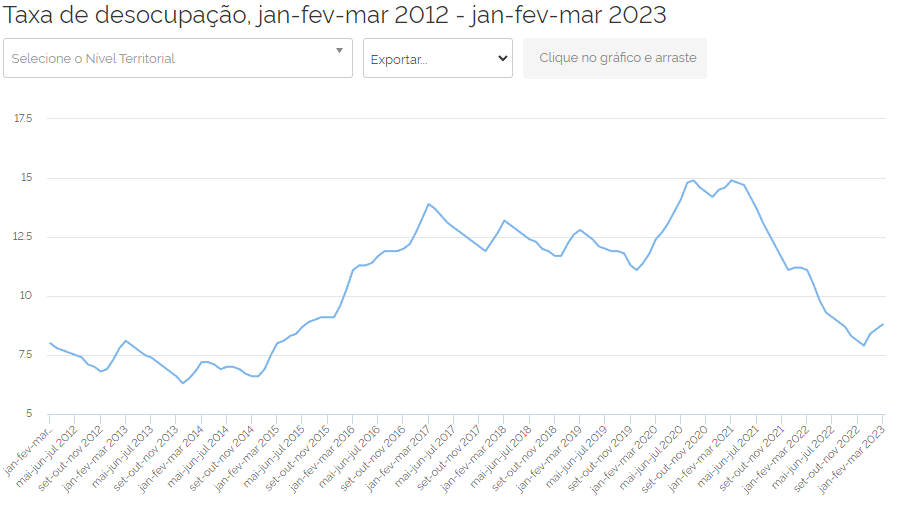
\includegraphics[width=\textwidth]{./figures/aula10_fig13.PNG}}};
			\end{tikzpicture}
			\tiny{{\scshape FIGURA}. \ Taxa de desocupação, Brasil (2012-2023). Fonte: \href{https://www.ibge.gov.br/estatisticas/sociais/trabalho/9173-pesquisa-nacional-por-amostra-de-domicilios-continua-trimestral.html?=&t=series-historicas&utm_source=landing&utm_medium=explica&utm_campaign=desemprego}{PNAD contínua - IBGE}} 
		\end{minipage}
	\end{center}
\end{frame}

\section{Determinação de Salários}
\begin{frame}
    {Determinação de salários: Introdução}
    \begin{itemize}
        \item Foco agora: determinação de salários e relação entre salários e desemprego\bigskip
        \item Salários podem ser fixados de várias formas\bigskip
        \item Podem ser determinados por \hlight{negociação coletiva}: negociação entre firmas e sindicatos\bigskip
        \item EUA: negociação coletiva tem papel limitado - $< 10\%$ dos trabalhadores com salários fixados por acordos coletivos\bigskip
        \item Para o restante dos trabalhadores, salários fixados ou por empregadores ou por negociações individuais\bigskip
        \item Quanto maior a qualificação necessária para o emprego, maior a probabilidade de haver negociação
    \end{itemize}
\end{frame}

\begin{frame}
    {Determinação de salários: Introdução}
    \begin{itemize}
        \item Diferenças entre países: e.g., negociação coletiva tem papel importante no Japão e maioria dos países europeus\bigskip
        \item Podem ser realizadas no nível das firmas, nível setorial ou nível nacional\bigskip
        \item Às vezes, acordos feitos por contrato aplicam-se apenas às empresas que assinaram o acordo\bigskip
        \item Outras, são estendidos automaticamente a todas as firmas e trabalhadores do setor ou da economia
    \end{itemize}
\end{frame}

\begin{frame}{Determinação de salários: Introdução}
    \begin{center}
		\begin{minipage}[b]{.55\textwidth}
			\begin{tikzpicture}
				\node[inner sep=0] (image) at (0,0) {\href{https://ilostat.ilo.org/topics/union-membership/}{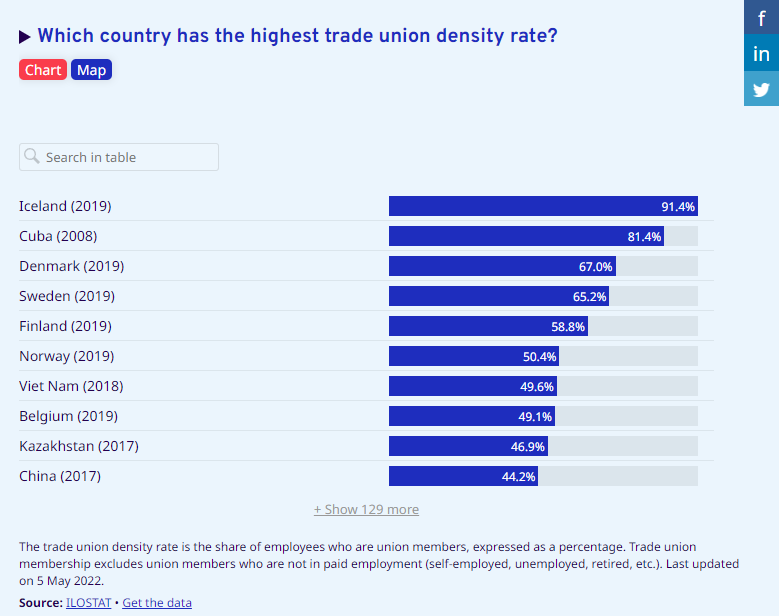
\includegraphics[width=\textwidth]{./figures/aula10_fig14.PNG}}};
			\end{tikzpicture}
			\tiny{{\scshape FIGURA}. \ Taxa de densidade de sindicatos. Fonte: \href{https://ilostat.ilo.org/topics/union-membership/}{ILOSTAT}} 
		\end{minipage}
	\end{center}
\end{frame}

\begin{frame}{Determinação de salários: Introdução}
    \begin{center}
		\begin{minipage}[b]{.6\textwidth}
			\begin{tikzpicture}
				\node[inner sep=0] (image) at (0,0) {\href{https://ilostat.ilo.org/topics/union-membership/}{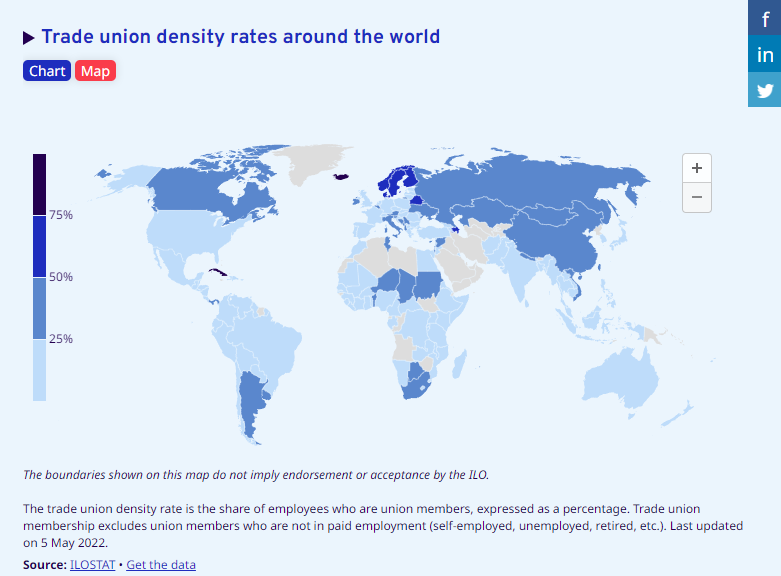
\includegraphics[width=\textwidth]{./figures/aula10_fig15.PNG}}};
			\end{tikzpicture}
			\tiny{{\scshape FIGURA}. \ Taxa de densidade de sindicatos. Fonte: \href{https://ilostat.ilo.org/topics/union-membership/}{ILOSTAT}} 
		\end{minipage}
	\end{center}
\end{frame}

\begin{frame}
    {Determinação de salários: Introdução}
    \emoji{question} Dadas diferenças entre trabalhadores e países, é possível formular uma teoria ``geral'' de determinação de salários\bigskip
    \begin{itemize}        
        \item Embora diferenças institucionais influenciem fixação de salários, há forças comuns em ação em todos os países\bigskip
        \item Dois conjuntos de fatores mais importantes:\medskip
        \begin{enumerate}
            \item Trabalhadores recebem salário que excede \textcolor{purple}{salário de reserva} (nível de salário que torna trabalhadores indiferentes entre trabalhar e permanecer desempregados)\medskip
            \item Salários normalmente dependem das condições do mercado de trabalho: quanto menor a taxa de desemprego, maiores os salários
        \end{enumerate}
    \end{itemize}
\end{frame}

\begin{frame}{Determinação de salários: Introdução}
    \begin{center}
		\begin{minipage}[b]{.8\textwidth}
			\begin{tikzpicture}
				\node[inner sep=0] (image) at (0,0) {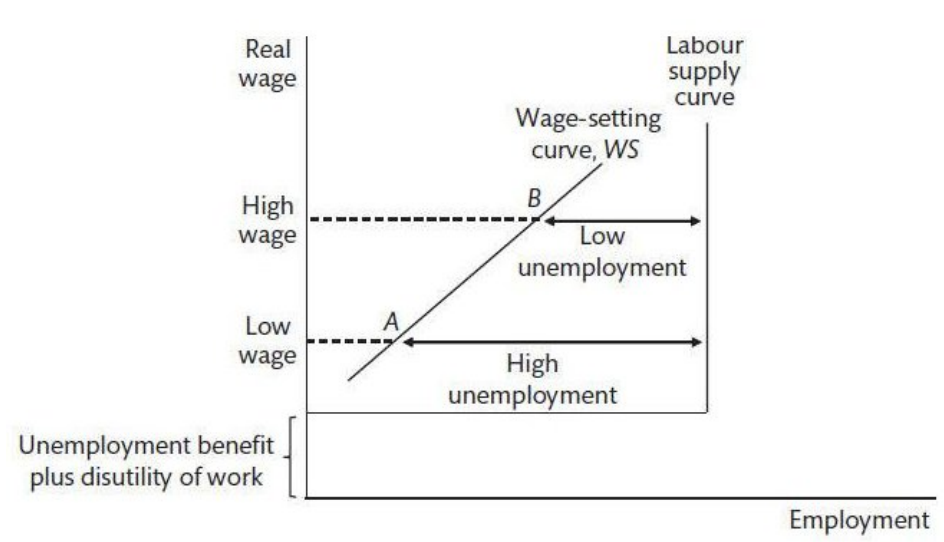
\includegraphics[width=\textwidth]{./figures/aula10_fig16.PNG}};
			\end{tikzpicture}
			\tiny{{\scshape FIGURA}. \ Curva de determinação de salários. Fonte: Carlin e Soskice (2015)} 
		\end{minipage}
	\end{center}
\end{frame}

\begin{frame}
    {Determinação de salários: introdução}
    \begin{itemize}
        \item Duas grandes linhas de raciocínio:\medskip
        \begin{enumerate}
            \item Mesmo na ausência de negociações coletivas, trabalhadores ainda tem algum poder de negociação que usam para obter uma remuneração superior ao salário de reserva\medskip
            \item Empresas podem, por vários motivos, desejar pagar remunerações mais altas que o salário de reserva
        \end{enumerate}
    \end{itemize}
\end{frame}
\section{Bibliografia}
\begin{frame}{\emoji{books} Bibliografia}
    \begin{itemize}                
        \item BLANCHARD, O. Macroeconomia. 7.ed. São Paulo: Pearson Education do Brasil, 2017\medskip                
        \item CARLIN, W.; SOSKICE, D. Macroeconomics: Institutions, instability, and the financial system. Oxford, UK: Oxford University Press, 2015\medskip
        \item CHALLE, E. Macroeconomic fluctuations and policies. Cambridge, MA: The MIT Press, 2019\medskip                
    \end{itemize}
\end{frame}
\end{document}